\documentclass{article}

\usepackage[margin=1.0in]{geometry}
\usepackage{graphicx}
\usepackage{amsmath}
\usepackage{float}
\usepackage{enumitem}

\title{CSC 535 HW9}
\date{12/06/2018}
\author{Simon Swenson}

\begin{document}

\pagenumbering{gobble}
\maketitle
\pagenumbering{arabic}

\section{Introduction}

All homework problems were completed. I was a little stumped on what an expected 
value of 24 cycles before a transition implied for the values within the 
transition matrix, for the cell problem. I settled on something that intuitively 
made sense to me, but 
it might not be the correct answer. Otherwise, I felt that 2.d and 2.e were very 
calculation heavy without much payoff in understanding. It was basically finding 
out how many of each probability to multiply, then multiply them all. Also, I 
suspect there's a high chance of human error in those problems, whereas those 
problems are much better suited to having a computer perform the computations.

\section{A Graphical Exploration of Hidden Markov Models}

\subsection{A State Transition Diagram Representing Progression Through College}

\begin{figure}[!ht]
	\centering
	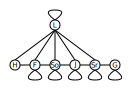
\includegraphics[width=120mm]{figs/college-progression.png}
	\caption{A state transition diagram representing progression through 
        college. Initially, a student is in high school (H) and chooses whether 
        to leave education (L) or continue to college (F). For each year in 
        college, freshman (F), sophmore (So), junior (J), and senior (Sr), the 
        student either passes his or her classes, and thus progresses to the 
        next year, or fails some or all of his or her classes. If he or she 
        fails classes, he or she must decide whether to continue his or her 
        education (thus remaining in the current year) or leave academia 
        altogether (L). If a student passes his or her senior (Sr) year, he 
        or she graduates (G) and remains a college graduate.}
\end{figure}

~\\
~\\
~\\
~\\
~\\
~\\
~\\
~\\
~\\
~\\
~\\
~\\
~\\
~\\
~\\
~\\
~\\
~\\
~\\
~\\
~\\
~\\
~\\
~\\
~\\
~\\
~\\
~\\

\subsection{A Hidden Markov Model for a Cell}

This scenario is a little interesting, because it concerns taking measurements 
at a different time interval than the actual state transitions. In addition, the 
measurements are for gene expressions rather than the underlying states. We 
could construct the model in terms of our measurement times (one hour intervals) 
or in terms of the actual state transition period (24 hours). Doing things in 
terms of measurements times gives us finer control over the state transition as 
well as provides a one set of outputs (gene expressions) per cycle. Since we 
want the expected value of the change to be after 24 cycles, we can cook up an 
equation to represent the probability that the organism has not changed state 
after 24 hours:

\begin{align*}
x^{24} &= 0.5 \\
x &\approx 0.97153 
\end{align*}

I chose 0.5 here because it seemed like the most reasonable mid-point between no 
chance and 100\% chance. I cannot explain it, but, intuitively, this seems like 
it would yield the correct expected value of 24 cycles. If it does not, I would 
love to hear in the feedback what the correct approach is. The transition matrix 
then becomes:

$$
T = \begin{bmatrix}
0.97153 & 0.02847 \\
0.02847 & 0.97153 \\
\end{bmatrix}
$$

The graph for the Hidden Markov Model is below. I list four observations for 
each cycle, representing the expression probability of each gene. I have come up 
with some 
arbitrary probabilities for those gene expressions.

\begin{figure}[!ht]
	\centering
	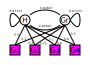
\includegraphics[width=120mm]{figs/cell-gene-expression.png}
	\caption{A graph for a HMM representing two cell states, hibernation and 
        growth, with a state transition time of one hour. For each of those 
        hours, a set of four genes are tested for whether they were expressed or 
        not. The probabilities of those genes being expressed is given as the 
        numbers next to the corresponding links.}
\end{figure}

\section{Reasoning About Trails}

\subsection{Trail Transition Matrix}

This is pretty straightforward. Each entry for an adjacent road is $\frac{1}{n}$, 
where $n$ is the number of adjacent roads. Let the rows represent the current 
hiker's location, sorted lexicographically, and let the columns represent the 
probabilities for the hiker's next location, sorted lexicographically. (The 
value for A is in entry 1, B in 2, and so on.)

$$
T = \begin{bmatrix}
0   & 1     & 0    & 0     & 0    & 0     & 0     & 0 \\
0.2 & 0     & 0.2  & 0.2   & 0.2  & 0     & 0.2   & 0 \\
0   & 0.333 & 0    & 0.333 & 0    & 0     & 0.333 & 0 \\
0   & 0.25  & 0.25 & 0     & 0    & 0.25  & 0.25  & 0 \\
0   & 0.333 & 0    & 0     & 0    & 0.333 & 0     & 0.333 \\
0   & 0     & 0    & 0.25  & 0.25 & 0     & 0.25  & 0.25 \\
0   & 0.25  & 0.25 & 0.25  & 0    & 0.25  & 0     & 0 \\
0   & 0     & 0    & 0     & 0.5  & 0.5   & 0     & 0
\end{bmatrix}
$$

\subsection{Is this a Markov Process?}

Markov Processes involve several key features. One is the change of state over 
time over a fininte number of states. States are represented by each fork in the 
trail. In addition, the transitions from a given state are a probability 
distribution. Thus, the rows in the transition matrix must sum to one. This is 
satisfied above. Markovian processes also assume that the only state that 
matters for determining the current state is the previous state. This is 
satisfied because the path transition probabilities are given only in terms of 
the current fork. One final observation is that this is a \textit{Hidden} Markov 
Model, since we can only reason about the state of the traveler based on 
indirect observations, in this case, the sensors, which are not perfect.

\subsection{Joint Probability of Observation Sequences}

First, define two observation output matrices as follows, where each row is a 
hidden state (current trail location), and each column is probability of the 
sensor output being $n$ at each location, given the hidden state. This is meant as 
an easy way to address a sensor output for a given hidden state.

$$
O_0 = \begin{bmatrix}
0.15 & 0.75 & 0.75 & 0.75 & 0.75 & 0.75 & 0.75 & 0.75 \\
0.75 & 0.15 & 0.75 & 0.75 & 0.75 & 0.75 & 0.75 & 0.75 \\
0.75 & 0.75 & 0.15 & 0.75 & 0.75 & 0.75 & 0.75 & 0.75 \\
0.75 & 0.75 & 0.75 & 0.15 & 0.75 & 0.75 & 0.75 & 0.75 \\
0.75 & 0.75 & 0.75 & 0.75 & 0.15 & 0.75 & 0.75 & 0.75 \\
0.75 & 0.75 & 0.75 & 0.75 & 0.75 & 0.15 & 0.75 & 0.75 \\
0.75 & 0.75 & 0.75 & 0.75 & 0.75 & 0.75 & 0.15 & 0.75 \\
0.75 & 0.75 & 0.75 & 0.75 & 0.75 & 0.75 & 0.75 & 0.15 \\
\end{bmatrix}
$$

$$
O_1 = \begin{bmatrix}
0.85 & 0.25 & 0.25 & 0.25 & 0.25 & 0.25 & 0.25 & 0.25 \\
0.25 & 0.85 & 0.25 & 0.25 & 0.25 & 0.25 & 0.25 & 0.25 \\
0.25 & 0.25 & 0.85 & 0.25 & 0.25 & 0.25 & 0.25 & 0.25 \\
0.25 & 0.25 & 0.25 & 0.85 & 0.25 & 0.25 & 0.25 & 0.25 \\
0.25 & 0.25 & 0.25 & 0.25 & 0.85 & 0.25 & 0.25 & 0.25 \\
0.25 & 0.25 & 0.25 & 0.25 & 0.25 & 0.85 & 0.25 & 0.25 \\
0.25 & 0.25 & 0.25 & 0.25 & 0.25 & 0.25 & 0.85 & 0.25 \\
0.25 & 0.25 & 0.25 & 0.25 & 0.25 & 0.25 & 0.25 & 0.85 \\
\end{bmatrix}
$$

You could also think of this as a tensor where $O_{i, j, k}$ represents the 
probability of the sensor output at fork $j$ being $k$, given the hidden state of $i$. As 
we are interested in a particular sequence output, I generated a sequence of 
state changes and observations by rolling some dice. We 
could write the probability of that sequence like this:

$$
\begin{gathered}
\pi_1    O_{1, 1, 1} O_{1, 2, 0} O_{1, 3, 1} O_{1, 4, 1} O_{1, 5, 0} O_{1, 6, 1} O_{1, 7, 0} O_{1, 8, 0} \\
T_{1, 2} O_{2, 1, 0} O_{2, 2, 1} O_{2, 3, 0} O_{2, 4, 1} O_{2, 5, 0} O_{2, 6, 0} O_{2, 7, 0} O_{2, 8, 1} \\
T_{2, 4} O_{4, 1, 0} O_{4, 2, 0} O_{4, 3, 1} O_{4, 4, 1} O_{4, 5, 0} O_{4, 6, 1} O_{4, 7, 0} O_{4, 8, 0} \\
\end{gathered}
$$

And so on, and so forth. Note that, in this case, $pi_1 = 1$, since the hiker 
\textit{always} starts at location A.

\subsection{Sensor Response Sequence Probabilities}

Given $R_1 = [a, b, c, d, b, c, d, b, e, f, h]$, what are the probabilities of 
the following sensor responses? For the following calcuations, I will make use 
of the tensor $O$ defined above.

\subsubsection{[\{a\}, \{b\}, \{c\}, \{d\}, \{b\}, \{c\}, \{d\}, \{b\}, \{e\}, \{f\}, \{h\}]}

$$
\begin{gathered}
P([\{a\}, \{b\}, \{c\}, \{d\}, \{b\}, \{c\}, \{d\}, \{b\}, \{e\}, \{f\}, \{h\}]) = \\
O_{1, 1, 1} O_{1, 2, 0}  O_{1, 3, 0}  O_{1, 4, 0}  O_{1, 5, 0}  O_{1, 6, 0}  O_{1, 7, 0}  O_{1, 8, 0} \\
O_{1, 1, 0} O_{1, 2, 1}  O_{1, 3, 0}  O_{1, 4, 0}  O_{1, 5, 0}  O_{1, 6, 0}  O_{1, 7, 0}  O_{1, 8, 0} \\
O_{1, 1, 0} O_{1, 2, 0}  O_{1, 3, 1}  O_{1, 4, 0}  O_{1, 5, 0}  O_{1, 6, 0}  O_{1, 7, 0}  O_{1, 8, 0} \\
O_{1, 1, 0} O_{1, 2, 0}  O_{1, 3, 0}  O_{1, 4, 1}  O_{1, 5, 0}  O_{1, 6, 0}  O_{1, 7, 0}  O_{1, 8, 0} \\
O_{1, 1, 0} O_{1, 2, 1}  O_{1, 3, 0}  O_{1, 4, 0}  O_{1, 5, 0}  O_{1, 6, 0}  O_{1, 7, 0}  O_{1, 8, 0} \\
O_{1, 1, 0} O_{1, 2, 0}  O_{1, 3, 1}  O_{1, 4, 0}  O_{1, 5, 0}  O_{1, 6, 0}  O_{1, 7, 0}  O_{1, 8, 0} \\
O_{1, 1, 0} O_{1, 2, 0}  O_{1, 3, 0}  O_{1, 4, 1}  O_{1, 5, 0}  O_{1, 6, 0}  O_{1, 7, 0}  O_{1, 8, 0} \\
O_{1, 1, 0} O_{1, 2, 1}  O_{1, 3, 0}  O_{1, 4, 0}  O_{1, 5, 0}  O_{1, 6, 0}  O_{1, 7, 0}  O_{1, 8, 0} \\
O_{1, 1, 0} O_{1, 2, 0}  O_{1, 3, 0}  O_{1, 4, 0}  O_{1, 5, 1}  O_{1, 6, 0}  O_{1, 7, 0}  O_{1, 8, 0} \\
O_{1, 1, 0} O_{1, 2, 0}  O_{1, 3, 0}  O_{1, 4, 0}  O_{1, 5, 0}  O_{1, 6, 1}  O_{1, 7, 0}  O_{1, 8, 0} \\
O_{1, 1, 0} O_{1, 2, 0}  O_{1, 3, 0}  O_{1, 4, 0}  O_{1, 5, 0}  O_{1, 6, 0}  O_{1, 7, 0}  O_{1, 8, 1} \\
= \\
0.85 \times 0.75 \times 0.75 \times 0.75 \times 0.75 \times 0.75 \times 0.75 \times 0.75 \\
0.75 \times 0.85 \times 0.75 \times 0.75 \times 0.75 \times 0.75 \times 0.75 \times 0.75 \\
0.75 \times 0.75 \times 0.85 \times 0.75 \times 0.75 \times 0.75 \times 0.75 \times 0.75 \\
0.75 \times 0.75 \times 0.75 \times 0.85 \times 0.75 \times 0.75 \times 0.75 \times 0.75 \\
0.75 \times 0.85 \times 0.75 \times 0.75 \times 0.75 \times 0.75 \times 0.75 \times 0.75 \\
0.75 \times 0.75 \times 0.85 \times 0.75 \times 0.75 \times 0.75 \times 0.75 \times 0.75 \\
0.75 \times 0.75 \times 0.75 \times 0.85 \times 0.75 \times 0.75 \times 0.75 \times 0.75 \\
0.75 \times 0.85 \times 0.75 \times 0.75 \times 0.75 \times 0.75 \times 0.75 \times 0.75 \\
0.75 \times 0.75 \times 0.75 \times 0.75 \times 0.85 \times 0.75 \times 0.75 \times 0.75 \\
0.75 \times 0.75 \times 0.75 \times 0.75 \times 0.75 \times 0.85 \times 0.75 \times 0.75 \\
0.75 \times 0.75 \times 0.75 \times 0.75 \times 0.75 \times 0.75 \times 0.75 \times 0.85 \\
=\\
0.85^{11} \times 0.75^{77} \approx 4.01167 \times 10^{-11}
\end{gathered}
$$

We expected this to be the expected value for all sensor outputs, but, even so, 
the space for all of these sensor outputs after 11 states is so large that we 
yield an incredibly small probability.

\subsubsection{[\{a, b\}, \{b, c\}, \{c, d\}, \{d, f\}, \{b, d\}, \{c, f\}, \{d, h\}, \{b, e\}, \{e, h\}, \{f, e\}, \{f, h\}]}

For the following sequence, if we're clever, we can recognize that it contains 
every \textit{actual} hidden state in addition to one false positive. There are 
thus 6 true negatives, 1 true positive, and 1 false positive for each of the 13 
states. We can use this to group the exponents:

$$
\begin{gathered}
P([\{a, b\}, \{b, c\}, \{c, d\}, \{d, f\}, \{b, d\}, \{c, f\}, \{d, h\}, \{b, e\}, \{e, h\}, \{f, e\}, \{f, h\}]) = \\
0.75^{66} \times 0.25^{11} \times 0.85^{11} \approx 2.26460 \times 10^{-16}
\end{gathered}
$$

Notice how just one false positive per state can reduce the probability by a 
substantial amount (by a factor of roughly a hundred thousand).

\subsubsection{[\{\}, \{b\}, \{\}, \{f\}, \{\}, \{f\}, \{\}, \{h\}, \{\}, \{e\}, \{\}]}

This sensor output sequence will probably have the lowest probability of all. 
There is only one true positive and several false positives. The sensors seemed to 
be taking a nap in this sequence.

$$
\begin{gathered}
P([\{\}, \{b\}, \{\}, \{f\}, \{\}, \{f\}, \{\}, \{h\}, \{\}, \{e\}, \{\}]) = \\
0.75^{73} \times 0.25^{4} \times 0.85 \times 0.15^{10} \approx 1.45065 \times 10^{-20}
\end{gathered}
$$

As expected, a very low probability. The ten false negatives really bring the 
probability for this sequence down.

\subsection{Same Sensor Responses, Different Sequence}

Now consider the hidden sequence $R_2 = [a, b, d, f, d, f, h, e, h, e, f]$ and 
the same sensor responses.

\subsubsection{[\{a\}, \{b\}, \{c\}, \{d\}, \{b\}, \{c\}, \{d\}, \{b\}, \{e\}, \{f\}, \{h\}]}

$$
\begin{gathered}
P([\{a\}, \{b\}, \{c\}, \{d\}, \{b\}, \{c\}, \{d\}, \{b\}, \{e\}, \{f\}, \{h\}]) = \\
0.75^{68} \times 0.25^{9} \times 0.85^{2} \times 0.15^{9} \approx 3.38287 \times 10^{-22}
\end{gathered}
$$

\subsubsection{[\{a, b\}, \{b, c\}, \{c, d\}, \{d, f\}, \{b, d\}, \{c, f\}, \{d, h\}, \{b, e\}, \{e, h\}, \{f, e\}, \{f, h\}]}

The astute observer will note that this sequence of sensor outputs includes all 
of the actual hidden states of the first sequence and the second sequence. This 
makes the probability for the two exactly the same. 

$$
\begin{gathered}
P([\{a, b\}, \{b, c\}, \{c, d\}, \{d, f\}, \{b, d\}, \{c, f\}, \{d, h\}, \{b, e\}, \{e, h\}, \{f, e\}, \{f, h\}]) = \\
0.75^{66} \times 0.25^{11} \times 0.85^{11} \approx 2.26460 \times 10^{-16}
\end{gathered}
$$

\subsubsection{[\{\}, \{b\}, \{\}, \{f\}, \{\}, \{f\}, \{\}, \{h\}, \{\}, \{e\}, \{\}]}

$$
\begin{gathered}
P([\{\}, \{b\}, \{\}, \{f\}, \{\}, \{f\}, \{\}, \{h\}, \{\}, \{e\}, \{\}]) = \\
0.75^{76} \times 0.25 \times 0.85^{4} \times 0.15^{7} \approx 7.12706 \times 10^{-17}
\end{gathered}
$$

\section{HMM: Other Possible Applications?}

\subsection{Can a HMM Work for Baby MQLs?}

For normal MQLs, movement seems very straightforward to model with a HMM. In the 
stationary state, they have a probability of staying in the stationary state (S), 
transitioning to the move left one state ("releasing the magnetic force on the 
left foot," what I will call ML1), or transitioning to the move 
right one state (MR1). According to the description, ML1 will transition to ML2 ("moving 
the left foot outward") with 100\% probability. Then, ML2 will transition to 
ML3 ("activating the [left foot] magnet") with 100\% probability. ML3 will 
transition to ML4 ("releasing the magnet on the right foot") with 100\% 
probability. ML4 will transition to ML5 ("drawing the legs together") with 100\% 
probability. ML5 will transition to S ("activating the right foot magnet") 
with 100\% probability. A similar sequence can represent movement rightward. 
Note that some of these actions taken in isolation 
appear when moving right, as well, but it is important to differentiate them, 
as, when we 
take the movement as a whole, the states transition in a very different way 
between leftwards movement and rightwards movement.

For baby MQLs, the story is actually not much different. However, instead of 
two paths which are relatively deterministic, there is some chance of branching. 
As it was not specified in the problem, I will assume that the baby MQL will 
continue the movement sequence even if its arm is up. Thus, unless the baby 
falls, it will take the same amount of moves to complete the movement. However, 
for all states with a magnet detached, there will be a second state 
corresponding to the baby losing its balance and raising its arm. For example, 
the state ML1B corresponds to the state when the baby has just started its 
journey leftward and has raised its left arm because its left leg's magnet 
became detached. The state transition diagram is below:

\begin{figure}[!ht]
	\centering
	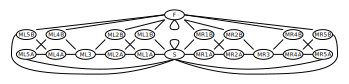
\includegraphics[width=160mm]{figs/baby-mql.png}
	\caption{A state transition diagram for the movement of a baby MQL. Nodes 
        ending in "B" represent movement when the baby is starting to lose its 
        balance and has thus raised its corresponding arm. Note that these 
        states can only happen when the MQL has deactivated one of its magnets. 
        "F" represents 
        being in the fallen state. "S" is the stationary state.}
\end{figure}

Note that not even this figure tells the whole story, as, at each state, we 
observe the MQL. Thus, each state would emit an angle for each of the MQL's 
inner legs, inner arms, outer legs, and outer arms. We might even measure body 
shape, as we did in a few assignments back. Each state would have a different 
probability distribution for each of these emittances.

\subsection{Can a HMM Work for a Malfunctioning Metronome?}

A normal metronome would be easy to model with a HMM, but, in this case, the 
failure rate is depedent on age. This means that, as the metronome ages, its 
transition probabilities also change. Unfortunately, 
this means that we do not have a constant transition matrix. Therefore, this 
scenario cannot be represented by a HMM.

\section{Conclusion}

HMMs are powerful for modeling state transitions over time. We have seen how 
they can be applied to model a student's progression (or lack thereof) through 
college, a cell's stages of hibernation and growth, a hiker's path through a web 
of trails, and a baby MQL's first steps. However, HMMs have 
some limitations. First, they can only represent a fininte number of states. 
This makes them efficient to implement using vectors and matrices, but, 
sometimes, real world scenarios require a continuous universe of states. Second, 
if transitions are represented as a matrix, each row in that matrix must 
correspond to a probability distribution and thus sum to one. Third, a 
first-order HMM assumes that a state only depends on the immediately previous 
state and no other states, which can be a shaky assumption to make in many 
scenarios. Fourth, the model is hidden in the fact that the \textit{true} state 
can only be inferred through a series of observations, which can have a variety 
of probability distributions. Last, the trasition matrix must remain constant 
throughout all of the transitions.

\end{document}